\documentclass{standalone}
\usepackage{tikz}
\begin{document}
% Created by tikzDevice version 0.7.0 on 2015-04-23 13:29:27
% !TEX encoding = UTF-8 Unicode
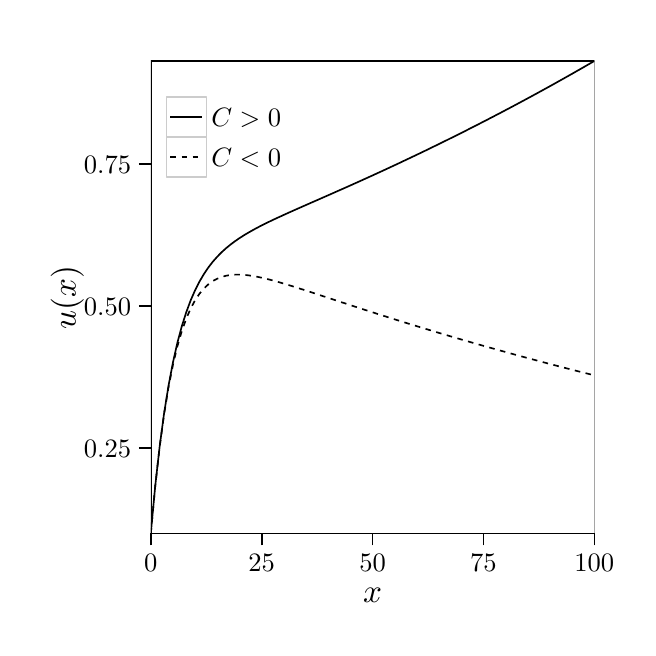
\begin{tikzpicture}[x=1pt,y=1pt]
\definecolor[named]{fillColor}{rgb}{1.00,1.00,1.00}
\path[use as bounding box,fill=fillColor,fill opacity=0.00] (0,0) rectangle (216.81,216.81);
\begin{scope}
\path[clip] (  0.00,  0.00) rectangle (216.81,216.81);
\definecolor[named]{drawColor}{rgb}{1.00,1.00,1.00}
\definecolor[named]{fillColor}{rgb}{1.00,1.00,1.00}

\path[draw=drawColor,line width= 0.6pt,line join=round,line cap=round,fill=fillColor] ( -0.00,  0.00) rectangle (216.81,216.81);
\end{scope}
\begin{scope}
\path[clip] ( 44.49, 34.03) rectangle (204.76,204.77);
\definecolor[named]{fillColor}{rgb}{1.00,1.00,1.00}

\path[fill=fillColor] ( 44.49, 34.03) rectangle (204.76,204.77);
\definecolor[named]{drawColor}{rgb}{0.00,0.00,0.00}

\path[draw=drawColor,line width= 0.6pt,line join=round] ( 44.49, 34.03) --
	( 46.09, 51.17) --
	( 47.69, 65.48) --
	( 49.29, 77.44) --
	( 50.90, 87.47) --
	( 52.50, 95.88) --
	( 54.10,102.97) --
	( 55.70,108.94) --
	( 57.31,114.00) --
	( 58.91,118.30) --
	( 60.51,121.97) --
	( 62.12,125.12) --
	( 63.72,127.84) --
	( 65.32,130.20) --
	( 66.92,132.27) --
	( 68.53,134.08) --
	( 70.13,135.70) --
	( 71.73,137.15) --
	( 73.34,138.46) --
	( 74.94,139.66) --
	( 76.54,140.76) --
	( 78.14,141.78) --
	( 79.75,142.74) --
	( 81.35,143.65) --
	( 82.95,144.52) --
	( 84.56,145.35) --
	( 86.16,146.15) --
	( 87.76,146.93) --
	( 89.36,147.69) --
	( 90.97,148.43) --
	( 92.57,149.16) --
	( 94.17,149.89) --
	( 95.77,150.61) --
	( 97.38,151.32) --
	( 98.98,152.03) --
	(100.58,152.73) --
	(102.19,153.44) --
	(103.79,154.14) --
	(105.39,154.84) --
	(106.99,155.55) --
	(108.60,156.25) --
	(110.20,156.96) --
	(111.80,157.67) --
	(113.41,158.38) --
	(115.01,159.09) --
	(116.61,159.80) --
	(118.21,160.52) --
	(119.82,161.24) --
	(121.42,161.97) --
	(123.02,162.69) --
	(124.63,163.42) --
	(126.23,164.16) --
	(127.83,164.89) --
	(129.43,165.63) --
	(131.04,166.38) --
	(132.64,167.12) --
	(134.24,167.87) --
	(135.84,168.63) --
	(137.45,169.39) --
	(139.05,170.15) --
	(140.65,170.91) --
	(142.26,171.68) --
	(143.86,172.45) --
	(145.46,173.23) --
	(147.06,174.01) --
	(148.67,174.79) --
	(150.27,175.58) --
	(151.87,176.37) --
	(153.48,177.17) --
	(155.08,177.97) --
	(156.68,178.77) --
	(158.28,179.57) --
	(159.89,180.39) --
	(161.49,181.20) --
	(163.09,182.02) --
	(164.70,182.84) --
	(166.30,183.67) --
	(167.90,184.50) --
	(169.50,185.33) --
	(171.11,186.17) --
	(172.71,187.02) --
	(174.31,187.86) --
	(175.91,188.71) --
	(177.52,189.57) --
	(179.12,190.43) --
	(180.72,191.29) --
	(182.33,192.16) --
	(183.93,193.03) --
	(185.53,193.91) --
	(187.13,194.79) --
	(188.74,195.67) --
	(190.34,196.56) --
	(191.94,197.46) --
	(193.55,198.36) --
	(195.15,199.26) --
	(196.75,200.16) --
	(198.35,201.08) --
	(199.96,201.99) --
	(201.56,202.91) --
	(203.16,203.84) --
	(204.76,204.77);

\path[draw=drawColor,line width= 0.6pt,dash pattern=on 2pt off 2pt ,line join=round] ( 44.49, 34.03) --
	( 46.09, 51.13) --
	( 47.69, 65.35) --
	( 49.29, 77.15) --
	( 50.90, 86.94) --
	( 52.50, 95.03) --
	( 54.10,101.71) --
	( 55.70,107.19) --
	( 57.31,111.69) --
	( 58.91,115.36) --
	( 60.51,118.33) --
	( 62.12,120.71) --
	( 63.72,122.61) --
	( 65.32,124.10) --
	( 66.92,125.26) --
	( 68.53,126.12) --
	( 70.13,126.75) --
	( 71.73,127.18) --
	( 73.34,127.44) --
	( 74.94,127.57) --
	( 76.54,127.58) --
	( 78.14,127.49) --
	( 79.75,127.32) --
	( 81.35,127.08) --
	( 82.95,126.79) --
	( 84.56,126.46) --
	( 86.16,126.08) --
	( 87.76,125.68) --
	( 89.36,125.24) --
	( 90.97,124.79) --
	( 92.57,124.32) --
	( 94.17,123.84) --
	( 95.77,123.34) --
	( 97.38,122.84) --
	( 98.98,122.32) --
	(100.58,121.81) --
	(102.19,121.29) --
	(103.79,120.76) --
	(105.39,120.24) --
	(106.99,119.71) --
	(108.60,119.18) --
	(110.20,118.65) --
	(111.80,118.13) --
	(113.41,117.60) --
	(115.01,117.07) --
	(116.61,116.55) --
	(118.21,116.03) --
	(119.82,115.50) --
	(121.42,114.98) --
	(123.02,114.47) --
	(124.63,113.95) --
	(126.23,113.44) --
	(127.83,112.93) --
	(129.43,112.42) --
	(131.04,111.91) --
	(132.64,111.41) --
	(134.24,110.91) --
	(135.84,110.41) --
	(137.45,109.91) --
	(139.05,109.42) --
	(140.65,108.93) --
	(142.26,108.44) --
	(143.86,107.95) --
	(145.46,107.47) --
	(147.06,106.98) --
	(148.67,106.50) --
	(150.27,106.03) --
	(151.87,105.55) --
	(153.48,105.08) --
	(155.08,104.61) --
	(156.68,104.14) --
	(158.28,103.68) --
	(159.89,103.21) --
	(161.49,102.75) --
	(163.09,102.30) --
	(164.70,101.84) --
	(166.30,101.39) --
	(167.90,100.94) --
	(169.50,100.49) --
	(171.11,100.04) --
	(172.71, 99.60) --
	(174.31, 99.15) --
	(175.91, 98.71) --
	(177.52, 98.28) --
	(179.12, 97.84) --
	(180.72, 97.41) --
	(182.33, 96.98) --
	(183.93, 96.55) --
	(185.53, 96.12) --
	(187.13, 95.70) --
	(188.74, 95.28) --
	(190.34, 94.86) --
	(191.94, 94.44) --
	(193.55, 94.02) --
	(195.15, 93.61) --
	(196.75, 93.20) --
	(198.35, 92.79) --
	(199.96, 92.38) --
	(201.56, 91.98) --
	(203.16, 91.58) --
	(204.76, 91.18);

\path[draw=drawColor,line width= 0.6pt,line join=round,line cap=round] ( 44.49, 34.03) rectangle (204.76,204.77);
\end{scope}
\begin{scope}
\path[clip] (  0.00,  0.00) rectangle (216.81,216.81);
\definecolor[named]{drawColor}{rgb}{0.00,0.00,0.00}

\node[text=drawColor,anchor=base east,inner sep=0pt, outer sep=0pt, scale=  0.96] at ( 37.37, 61.54) {0.25};

\node[text=drawColor,anchor=base east,inner sep=0pt, outer sep=0pt, scale=  0.96] at ( 37.37,112.88) {0.50};

\node[text=drawColor,anchor=base east,inner sep=0pt, outer sep=0pt, scale=  0.96] at ( 37.37,164.23) {0.75};
\end{scope}
\begin{scope}
\path[clip] (  0.00,  0.00) rectangle (216.81,216.81);
\definecolor[named]{drawColor}{rgb}{0.00,0.00,0.00}

\path[draw=drawColor,line width= 0.6pt,line join=round] ( 40.22, 64.84) --
	( 44.49, 64.84);

\path[draw=drawColor,line width= 0.6pt,line join=round] ( 40.22,116.19) --
	( 44.49,116.19);

\path[draw=drawColor,line width= 0.6pt,line join=round] ( 40.22,167.53) --
	( 44.49,167.53);
\end{scope}
\begin{scope}
\path[clip] (  0.00,  0.00) rectangle (216.81,216.81);
\definecolor[named]{drawColor}{rgb}{0.00,0.00,0.00}

\path[draw=drawColor,line width= 0.6pt,line join=round] ( 44.49, 29.77) --
	( 44.49, 34.03);

\path[draw=drawColor,line width= 0.6pt,line join=round] ( 84.56, 29.77) --
	( 84.56, 34.03);

\path[draw=drawColor,line width= 0.6pt,line join=round] (124.63, 29.77) --
	(124.63, 34.03);

\path[draw=drawColor,line width= 0.6pt,line join=round] (164.70, 29.77) --
	(164.70, 34.03);

\path[draw=drawColor,line width= 0.6pt,line join=round] (204.76, 29.77) --
	(204.76, 34.03);
\end{scope}
\begin{scope}
\path[clip] (  0.00,  0.00) rectangle (216.81,216.81);
\definecolor[named]{drawColor}{rgb}{0.00,0.00,0.00}

\node[text=drawColor,anchor=base,inner sep=0pt, outer sep=0pt, scale=  0.96] at ( 44.49, 20.31) {0};

\node[text=drawColor,anchor=base,inner sep=0pt, outer sep=0pt, scale=  0.96] at ( 84.56, 20.31) {25};

\node[text=drawColor,anchor=base,inner sep=0pt, outer sep=0pt, scale=  0.96] at (124.63, 20.31) {50};

\node[text=drawColor,anchor=base,inner sep=0pt, outer sep=0pt, scale=  0.96] at (164.70, 20.31) {75};

\node[text=drawColor,anchor=base,inner sep=0pt, outer sep=0pt, scale=  0.96] at (204.76, 20.31) {100};
\end{scope}
\begin{scope}
\path[clip] (  0.00,  0.00) rectangle (216.81,216.81);
\definecolor[named]{drawColor}{rgb}{0.00,0.00,0.00}

\node[text=drawColor,anchor=base,inner sep=0pt, outer sep=0pt, scale=  1.20] at (124.63,  9.03) {$x$};
\end{scope}
\begin{scope}
\path[clip] (  0.00,  0.00) rectangle (216.81,216.81);
\definecolor[named]{drawColor}{rgb}{0.00,0.00,0.00}

\node[text=drawColor,rotate= 90.00,anchor=base,inner sep=0pt, outer sep=0pt, scale=  1.20] at ( 17.30,119.40) {$u(x)$};
\end{scope}
\begin{scope}
\path[clip] (  0.00,  0.00) rectangle (216.81,216.81);
\definecolor[named]{fillColor}{rgb}{1.00,1.00,1.00}

\path[fill=fillColor] ( 45.88,158.63) rectangle (107.20,199.68);
\end{scope}
\begin{scope}
\path[clip] (  0.00,  0.00) rectangle (216.81,216.81);
\definecolor[named]{drawColor}{rgb}{0.80,0.80,0.80}
\definecolor[named]{fillColor}{rgb}{1.00,1.00,1.00}

\path[draw=drawColor,line width= 0.6pt,line join=round,line cap=round,fill=fillColor] ( 50.15,177.35) rectangle ( 64.60,191.80);
\end{scope}
\begin{scope}
\path[clip] (  0.00,  0.00) rectangle (216.81,216.81);
\definecolor[named]{drawColor}{rgb}{0.00,0.00,0.00}

\path[draw=drawColor,line width= 0.6pt,line join=round] ( 51.59,184.58) -- ( 63.16,184.58);
\end{scope}
\begin{scope}
\path[clip] (  0.00,  0.00) rectangle (216.81,216.81);
\definecolor[named]{drawColor}{rgb}{0.80,0.80,0.80}
\definecolor[named]{fillColor}{rgb}{1.00,1.00,1.00}

\path[draw=drawColor,line width= 0.6pt,line join=round,line cap=round,fill=fillColor] ( 50.15,162.89) rectangle ( 64.60,177.35);
\end{scope}
\begin{scope}
\path[clip] (  0.00,  0.00) rectangle (216.81,216.81);
\definecolor[named]{drawColor}{rgb}{0.00,0.00,0.00}

\path[draw=drawColor,line width= 0.6pt,dash pattern=on 2pt off 2pt ,line join=round] ( 51.59,170.12) -- ( 63.16,170.12);
\end{scope}
\begin{scope}
\path[clip] (  0.00,  0.00) rectangle (216.81,216.81);
\definecolor[named]{drawColor}{rgb}{0.00,0.00,0.00}

\node[text=drawColor,anchor=base west,inner sep=0pt, outer sep=0pt, scale=  0.96] at ( 66.41,181.27) {$C > 0$};
\end{scope}
\begin{scope}
\path[clip] (  0.00,  0.00) rectangle (216.81,216.81);
\definecolor[named]{drawColor}{rgb}{0.00,0.00,0.00}

\node[text=drawColor,anchor=base west,inner sep=0pt, outer sep=0pt, scale=  0.96] at ( 66.41,166.82) {$C < 0 $};
\end{scope}
\end{tikzpicture}
\end{document}
